\documentclass[11pt]{article}
%\usepackage{fontspec}
%\setmainfont{Arial}
\usepackage{helvet}
\renewcommand{\familydefault}{\sfdefault}
\usepackage[]{lipsum}
\usepackage{setspace,listings,color}
\setstretch{1.15}
\usepackage[a4paper, margin = 25.4mm]{geometry}
\usepackage[hidelinks]{hyperref}
\usepackage{lineno}
\linenumbers
\renewcommand\linenumberfont{\normalfont}
\usepackage{siunitx}
\usepackage{graphicx}
\usepackage{booktabs}
\usepackage{caption}
\usepackage{subcaption}
\usepackage{amsmath,amssymb,amsfonts,physics}
\usepackage{float}
\usepackage[numbers]{natbib}
\setlength{\parindent}{0pt}
\renewcommand{\bibsection}{}
\begin{document}
MECH0059: Advanced Computer Applications in Engineering

\textbf{Finite Element Analysis - Assignment}
\\
\\
Hasha Dar$^1$
\\
\\
$^1$Department of Mechanical Engineering, University College London, Torrington Place, London WC1E 7JE, UK
\\
\\
Student number: 19090799
\\
\\
\today
\\
\\
Word count:
\newpage
\textbf{Abstract:}
This assignment investigates the use of finite element analysis (FEA) to analyse a 2-D plate with a notch-shaped indentation under a plane stress condition. The aim of the assignment is to understand how commercial FEA packages operate from a low-level mathematical perspective. I utilise the finite element method for this analysis to determine the displacement and strain for a variety of Young's Moduli and loading conditions. The assignment stipulates to build a MATLAB programme to compute these variables. To investigate the accuracy of the programme, I replicate the problem in a commercially available FEA package, ANSYS Mechanical APDL, and gather the results for comparison and discussion.
\\
\\
\textbf{Key words:} finite element analysis, finite element method, 2-D plate, plane stress
\\
\\
\textbf{Introduction:}
Finite element analysis (FEA) is used to analyse the behaviour of components under certain conditions using the finite element method (FEM). This analysis encompasses a broad scope of physical phenomena, for example, deformation (elastic and plastic), modal analysis and thermal conduction \cite{twi}. Many of these problems involve the formulation of partial differential equations that are difficult to solve analytically, if at all possible. The introduction of the finite element method has since been able to solve these problems through discretisation \cite{KNOWLES1984134}. This is where a domain may be split up through the construction of a mesh into a number of elements, consisting of an assemblage of nodes. Hence, by defining the boundary conditions of a specific problem, a series of algebraic equations are generated, which can be solved numerically. Originally conceived to aid in structural analysis, FEM has widespread use in other areas of computer aided engineering (CAE), such as biomechanics and electromagnetic field problems \cite{seshu2003textbook}. We must also note that the use of the FEM to conduct these analyses is not a precise solution, rather a numerical approximation of the underlying partial differential equations that may define a physical system.
\\
\\
Due to the complexity and large size of the calculations typical in FEA, historically FEA packages have been developed specifically for use by commercial server grade computers i.e., commercial mainframes and super-computer clusters. In the last decade, the computing power available on personal computers has risen to a level permitting the use of commercial FEA packages \cite{AKIN198619}. This assignment aims to create a bare-bones programme within MATLAB to calculate the nodal displacements and strains for a thin plate.
\\
\\
\textbf{Methods:}

\textbf{\textit{Geometry and material properties:}} A 2-D plate with a notch indentation thin plate ($t = \SI{2}{mm}$) under a plane stress condition was used for the purposes of this investigation. The Young's Modulus of the material was set as $E=\SI{40}{GPa}$ in the base case and Poisson ratio $\nu = 0.3$. The geometry is shown in Figure \ref{geom}. This domain was discretised into four elements. Four-node quadrilateral elements were used in this analysis and the coordinates of these nodes is shown in Table \ref{nodeGeom}.

\textbf{\textit{Boundary conditions:}} Nodes 1 and 3 were constrained in x- and y- dimensions to zero displacement (fixed support). A pressure load acting normal to the surface in the positive x direction was applied to the right-hand vertical surface with magnitude \SI{200}{MPa}. This was discretised into three point loads acting on nodes 5,6,7 with magnitudes \SI{3000}{\newton}, \SI{6000}{\newton}, \SI{3000}{\newton} respectively.

\textbf{\textit{Part 1:}} MATLAB was used to write a code to compute the nodal displacement and elemental strains of the geometry. First, nodal geometry was stored in a 3-D matrix, where the 3rd dimension represents element number. Second, the shape functions were found and used to translate the geometry into a $\xi$-$\eta$ reference frame. Note, per element, the nodes are being referenced from the bottom left (index = 1) in a clockwise rotation.

\begin{equation}
    N = \begin{bmatrix}
        \dfrac{1}{4}\left(1-\xi\right)\left(1-\eta\right); &
        \dfrac{1}{4}\left(1-\xi\right)\left(1+\eta\right); &
        \dfrac{1}{4}\left(1+\xi\right)\left(1+\eta\right); &
        \dfrac{1}{4}\left(1+\xi\right)\left(1-\eta\right)
    \end{bmatrix}
\end{equation}

Sampling points (weighting factor: 1):

\begin{equation}
    \xi = \begin{bmatrix}
        -\dfrac{1}{\sqrt{3}}; &
        -\dfrac{1}{\sqrt{3}}; &
        \dfrac{1}{\sqrt{3}};  &
        \dfrac{1}{\sqrt{3}}
    \end{bmatrix}\qquad \eta = \begin{bmatrix}
        -\dfrac{1}{\sqrt{3}}; &
        \dfrac{1}{\sqrt{3}};  &
        \dfrac{1}{\sqrt{3}};  &
        -\dfrac{1}{\sqrt{3}}
    \end{bmatrix}
\end{equation}

From these, we can calculate our Jacobian matrices using \eqref{jacobian}. This relates the derivatives in the two coordinate frames.

\begin{equation}\label{jacobian}
    J = \begin{bmatrix}
        \sum \dfrac{\partial N_i}{\partial \xi}x_i  & \sum \dfrac{\partial N_i}{\partial \xi}y_i  \\
        \sum \dfrac{\partial N_i}{\partial \eta}x_i & \sum \dfrac{\partial N_i}{\partial \eta}y_i \\
    \end{bmatrix}
\end{equation}

Third, the $B$ matrix was formulated and computed.

\begin{align}
    B_1 & = \begin{bmatrix}
        1 & 0 & 0 & 0 \\
        0 & 0 & 0 & 1 \\
        0 & 1 & 1 & 0
    \end{bmatrix} \\
    B_2 & = \begin{bmatrix}
        \dfrac{J_{22}}{\abs{J}}  & -\dfrac{J_{12}}{\abs{J}} & 0                        & 0                        \\
        -\dfrac{J_{21}}{\abs{J}} & \dfrac{J_{11}}{\abs{J}}  & 0                        & 0                        \\
        0                        & 0                        & \dfrac{J_{22}}{\abs{J}}  & -\dfrac{J_{12}}{\abs{J}} \\
        0                        & 0                        & -\dfrac{J_{21}}{\abs{J}} & \dfrac{J_{11}}{\abs{J}}
    \end{bmatrix} \\
    B_3 & =\begin{bmatrix}
        \dfrac{\partial N_1}{\partial \xi}  & 0                                   & \dfrac{\partial N_2}{\partial \xi}  & 0                                   & \dfrac{\partial N_3}{\partial \xi}  & 0                                   & \dfrac{\partial N_4}{\partial \xi}  & 0                                   \\
        \dfrac{\partial N_1}{\partial \eta} & 0                                   & \dfrac{\partial N_2}{\partial \eta} & 0                                   & \dfrac{\partial N_3}{\partial \eta} & 0                                   & \dfrac{\partial N_4}{\partial \eta} & 0                                   \\
        0                                   & \dfrac{\partial N_1}{\partial \xi}  & 0                                   & \dfrac{\partial N_2}{\partial \xi}  & 0                                   & \dfrac{\partial N_3}{\partial \xi}  & 0                                   & \dfrac{\partial N_4}{\partial \xi}  \\
        0                                   & \dfrac{\partial N_1}{\partial \eta} & 0                                   & \dfrac{\partial N_2}{\partial \eta} & 0                                   & \dfrac{\partial N_3}{\partial \eta} & 0                                   & \dfrac{\partial N_4}{\partial \eta} \\
    \end{bmatrix}  \\
    B   & = B_1 B_2 B_3
\end{align}

Fourth, the $D$ matrix defines our material properties:

\begin{equation}
    D = \dfrac{E}{1-\nu^2}\begin{bmatrix}
        1   & \nu & 0                \\
        \nu & 1   & 0                \\
        0   & 0   & \dfrac{1-\nu}{2}
    \end{bmatrix}
\end{equation}

Fifth, the stiffness matrix per element can be computed:

\begin{equation}
    K_{element} = \int_{-1}^1\int_{-1}^1 B^T D B t\abs{J} \textrm{d}\xi\textrm{d}\eta
\end{equation}

Using Gauss quadrature rule, we can rewrite this equation as:

\begin{equation}
    K_{element} = \sum_i\sum_j\left(B^T D B t \abs{J}\right) W_i W_j
\end{equation}

Where the items in the parentheses are evaluated at each ($\xi_i$,$\eta_i$). These were then assembled into a global stiffness matrix with size $20\times 20$, representing $u$ and $v$ displacements for 10 nodes in x- and y- directions respectively. The elemental strain can be calculated using the nodal displacement and the following formulation:

\begin{equation}
    \varepsilon = B \delta_{element}
\end{equation}

where $\varepsilon$ is the elemental strain, $B$ is defined previously and $\delta_{element}$ are the nodal displacements for a given element.

\textbf{\textit{Part 2:}} The MATLAB code was amended and rerun to gather data for additional cases, namely: $E=\SI{10}{GPa}$, $E=\SI{100}{GPa}$, $E=\SI{200}{GPa}$ and $\alpha = \SI{30}{\degree}$, $\alpha = \SI{60}{\degree}$, $\alpha= \SI{135}{\degree}$.

\textbf{\textit{Part 3:}} The commercial package used to validate the results was ANSYS Mechanical APDL. The base case ($E = \SI{40}{GPa}, \alpha = \SI{90}{\degree}$) was used to validate the results.
\\
\\
\textbf{Results:}

\textbf{\textit{Part 1:}} The nodal displacement values in x- and y- directions ($u$ and $v$ respectively) are shown in Figure 2a. Here we see that node 2 has the highest vector sum displacement, peaking at a value of \SI{2.37e-04}{m}. Nodes 9 and 10 also exhibit high displacement and these correspond to the nodes at the portal of the notch. The elemental strains are shown in Figure 2B and show that elements 2 and 3 undergo relatively high amounts of y-axis strain and shear strain.

\textbf{\textit{Part 2:}} The nodal displacement in x- and y- directions for various Young's Moduli are shown in Figure 3. Here we see that for small values of $E$, there was greater displacement in both x- and y- directions. The nodal displacement in x- and y- for various angles of $\alpha$ are shown in Figure 4. Here we see the relationship that the closer the angle to the x- or y- axis, the greater the displacement in that direction. For the x- dimension, we see that $\alpha = \SI{90}{\degree}$ has the greatest displacement and for the y- dimension, $\alpha = \SI{135}{\degree}$ has the the highest displacement.

\textbf{\textit{Part 3:}} Figure 6 shows the contour plot from the simulation conducted in ANSYS. The results generated were for the base case and compared with the results from the MATLAB code. These are tabulated in Table 2.
\\
\\
\textbf{Discussion:}
It is evident from the ANSYS results that the code is not functioning properly and is not calculating the displacement of the nodes correctly. There are large percentage value differences and the nodal displacements are an order of magnitude removed from the ANSYS results. However, we do see that some of our results may be considered valid, such as that our displacements do change consistently with what is expected for the case of changing the Young's Modulus. We also see that the changing the pressure angle gives us the intended effect of increasing or decreasing the displacement in the x- or y- dimension.
\\
\\
\textbf{Figures and tables legend:}

Figure \ref{geom}: geometry of plate.

Figure \ref{fig:base}: (a) magnitude of nodal displacement $u$ and $v$ per node. (b) strain components per element

Figure \ref{fig:case1}: (a) comparison of x-coordinate displacement for a variety of Young's Moduli. (b) comparison of y-coordinate displacement for a variety of Young's Moduli.

Figure \ref{fig:case2}: (a) comparison of x-coordinate displacement for a variety of pressure angles. (b) comparison of y-coordinate displacement for a variety of pressure angles.

Figure \ref{fig:case3}: (a) comparison of strain components per element for a variety of Young's Moduli. (b) comparison of strain components per element for a variety of pressure angles.

Figure \ref{fig:case4}: contour plot of displacement for base case $E = \SI{40}{GPa}$ and $\alpha = \SI{90}{\degree}$.

Table \ref{nodeGeom}: tabulation of node geometries.

Table 2: tabulation of MATLAB and ANSYS nodal displacements with percentage error.
\\
\\
\textbf{References:}
\bibliographystyle{unsrtnat}
\bibliography{refs}
\newpage
\begin{figure}[H]
    \centering
    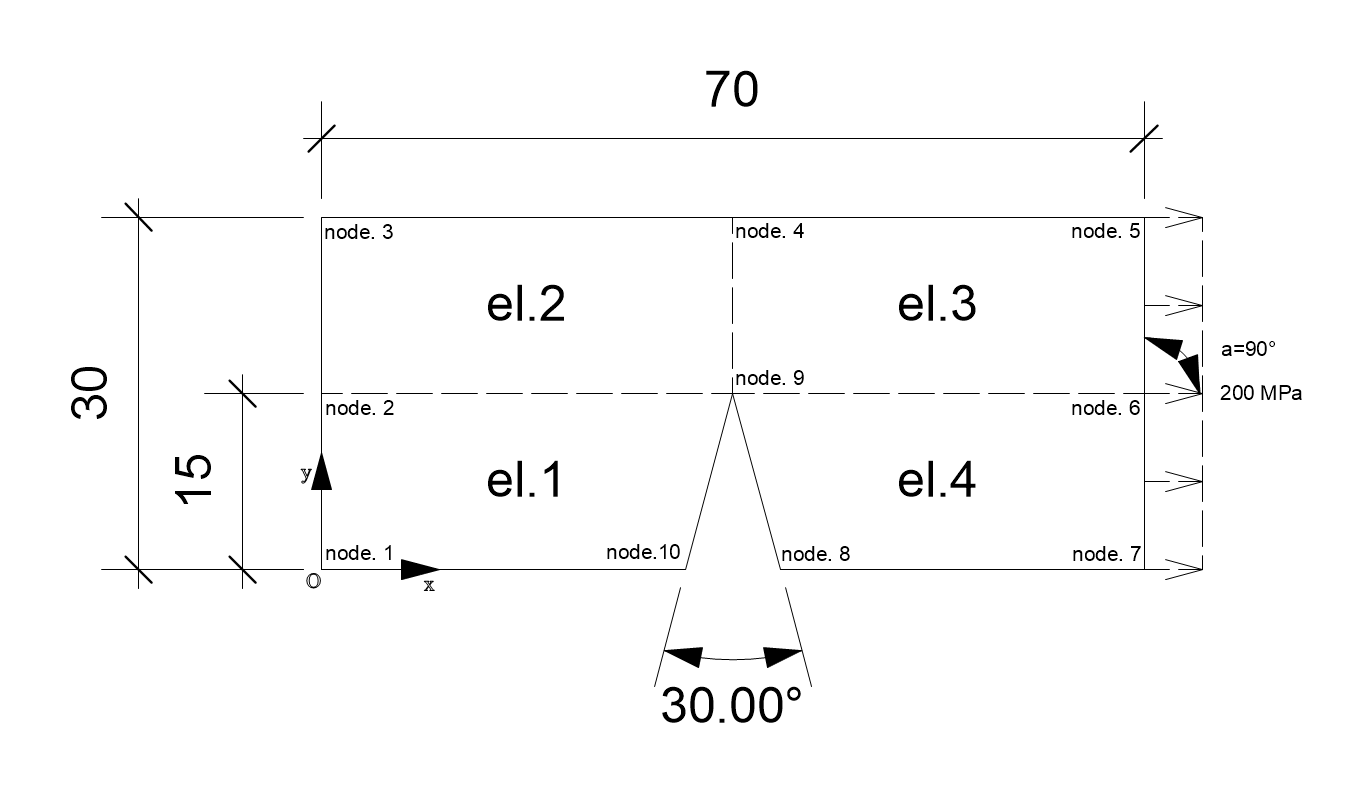
\includegraphics[width = 0.75\textwidth]{img/geom.png}
    \caption{}
    \label{geom}
\end{figure}
\begin{figure}[H]
    \centering
    \begin{subfigure}{.5\textwidth}
        \centering
        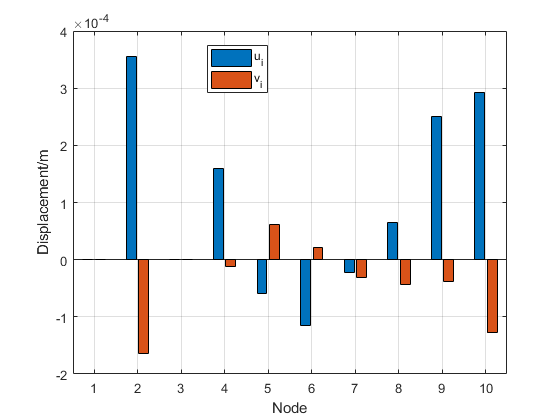
\includegraphics[width=\linewidth]{img/fig1}
        \caption{}
    \end{subfigure}%
    \begin{subfigure}{.5\textwidth}
        \centering
        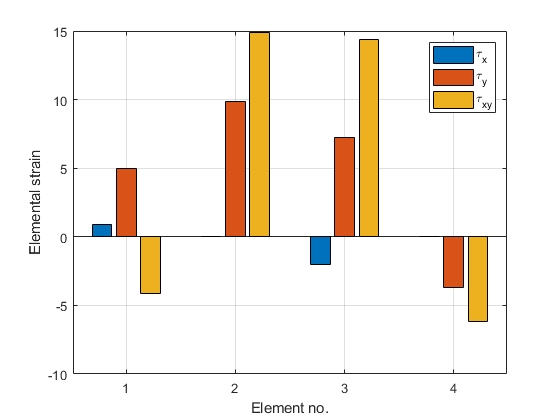
\includegraphics[width=\linewidth]{img/fig2}
        \caption{}
    \end{subfigure}
    \caption{}
    \label{fig:base}
\end{figure}
\begin{figure}[H]
    \centering
    \begin{subfigure}{.5\textwidth}
        \centering
        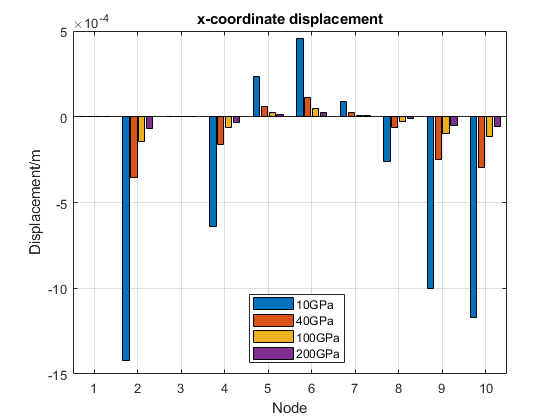
\includegraphics[width=\linewidth]{img/fig3}
        \caption{}
    \end{subfigure}%
    \begin{subfigure}{.5\textwidth}
        \centering
        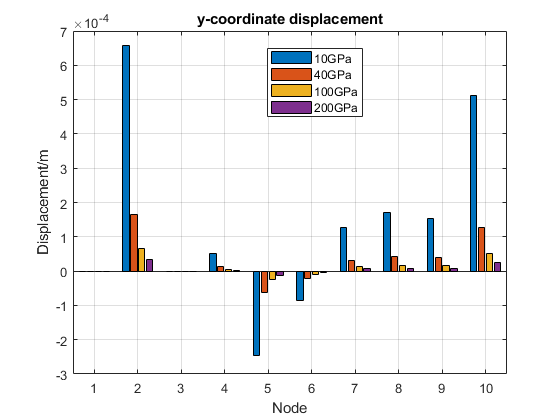
\includegraphics[width=\linewidth]{img/fig4}
        \caption{}
    \end{subfigure}
    \caption{}
    \label{fig:case1}
\end{figure}
\begin{figure}[H]
    \centering
    \begin{subfigure}{.5\textwidth}
        \centering
        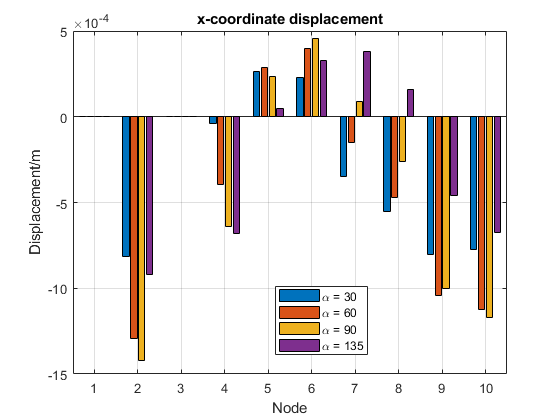
\includegraphics[width=\linewidth]{img/fig5}
        \caption{}
    \end{subfigure}%
    \begin{subfigure}{.5\textwidth}
        \centering
        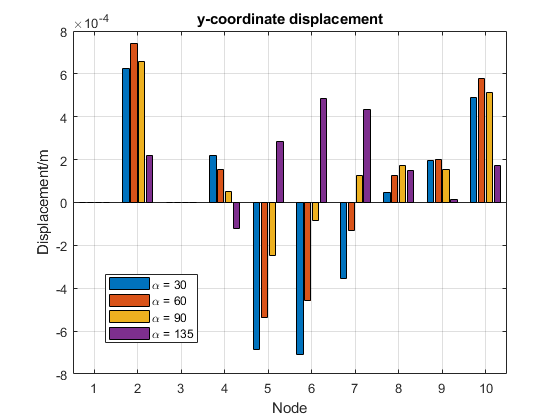
\includegraphics[width=\linewidth]{img/fig6}
        \caption{}
    \end{subfigure}
    \caption{}
    \label{fig:case2}
\end{figure}
\begin{figure}[H]
    \centering
    \begin{subfigure}{.5\textwidth}
        \centering
        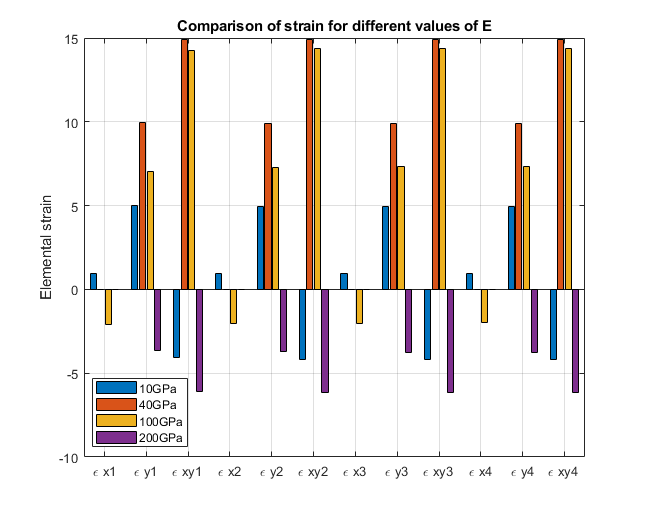
\includegraphics[width=\linewidth]{img/fig7}
        \caption{}
    \end{subfigure}%
    \begin{subfigure}{.5\textwidth}
        \centering
        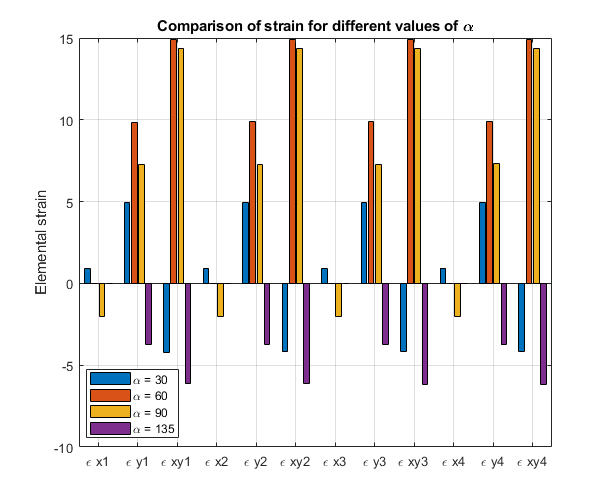
\includegraphics[width=\linewidth]{img/fig8}
        \caption{}
    \end{subfigure}
    \caption{}
    \label{fig:case3}
\end{figure}
\begin{figure}[H]
    \centering
    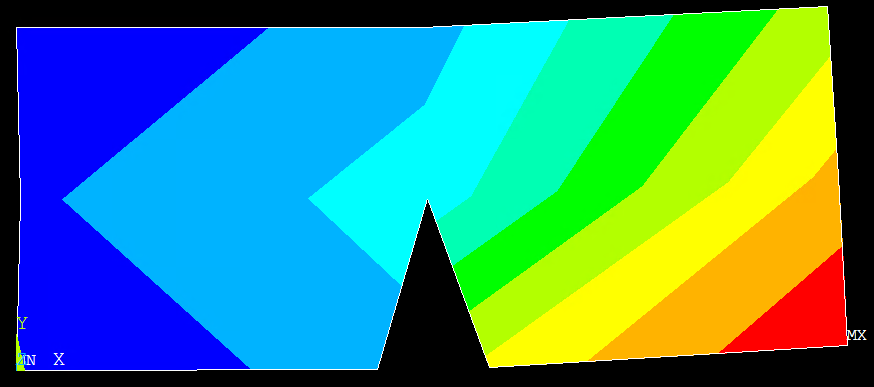
\includegraphics[width = 0.75\textwidth]{img/fig9.png}
    \caption{}
    \label{fig:case4}
\end{figure}
\begin{table}[H]
    \centering
    \begin{tabular}{@{}S[table-format=2.0]S[table-format=1.3]S[table-format=1.3]@{}}
        \toprule
        \textbf{Node} & \textbf{x-coordinate/m} & \textbf{y-coordinate/m} \\
        \midrule
        1             & 0.000                   & 0.000                   \\
        2             & 0.000                   & 0.015                   \\
        3             & 0.000                   & 0.030                   \\
        4             & 0.035                   & 0.030                   \\
        5             & 0.070                   & 0.030                   \\
        6             & 0.070                   & 0.015                   \\
        7             & 0.070                   & 0.000                   \\
        8             & 0.039                   & 0.000                   \\
        9             & 0.035                   & 0.015                   \\
        10            & 0.031                   & 0.000                   \\
        \bottomrule
    \end{tabular}
    \caption{}
    \label{nodeGeom}
\end{table}

% Please add the following required packages to your document preamble:
% \usepackage{booktabs}
\begin{table}[H]
    \centering
    \begin{tabular}{@{}cSSc@{}}
        \toprule
        \textbf{Variable} & \textbf{MATLAB displacement/m} & \textbf{ANSYS displacement/m} & \textbf{Percentage difference} \\
        \midrule
        $u1$              & 0.0E+00                        & 0.0E+00                       &                                \\
        $v1$              & 0.0E+00                        & 0.0E+00                       &                                \\
        $u2$              & -3.6E-04                       & 8.4E-05                       & -123.57\%                      \\
        $v2$              & 1.6E-04                        & 1.2E-06                       & -99.24\%                       \\
        $u3$              & 0.0E+00                        & 0.0E+00                       &                                \\
        $v3$              & 0.0E+00                        & 0.0E+00                       &                                \\
        $u4$              & -1.6E-04                       & 1.6E-04                       & -201.84\%                      \\
        $v4$              & 1.3E-05                        & 2.4E-06                       & -81.06\%                       \\
        $u5$              & 5.8E-05                        & 2.6E-04                       & 339.03\%                       \\
        $v5$              & -6.2E-05                       & 4.9E-04                       & -893.52\%                      \\
        $u6$              & 1.1E-04                        & 5.2E-04                       & 349.88\%                       \\
        $v6$              & -2.1E-05                       & 5.3E-04                       & -2570.43\%                     \\
        $u7$              & 2.3E-05                        & 7.1E-04                       & 3033.13\%                      \\
        $v7$              & 3.2E-05                        & 5.7E-04                       & 1698.52\%                      \\
        $u8$              & -6.5E-05                       & 6.3E-04                       & -1061.80\%                     \\
        $v7$              & 4.3E-05                        & 7.7E-05                       & 79.97\%                        \\
        $u9$              & -2.5E-04                       & 2.5E-04                       & -200.67\%                      \\
        $v9$              & 3.8E-05                        & 1.2E-05                       & -69.75\%                       \\
        $u10$             & -2.9E-04                       & 1.5E-04                       & -152.45\%                      \\
        $v10$             & 1.3E-04                        & 2.3E-05                       & -82.11\%                       \\ \bottomrule
    \end{tabular}
    \caption{}
\end{table}

\newpage
\textbf{Appendix:}
\appendix
\definecolor{dkgreen}{rgb}{0,0.6,0}
\definecolor{gray}{rgb}{0.5,0.5,0.5}
\definecolor{mauve}{rgb}{0.58,0,0.82}

\lstset{frame=tb,
    language=MATLAB,
    aboveskip=3mm,
    belowskip=3mm,
    showstringspaces=false,
    columns=flexible,
    basicstyle={\small\ttfamily},
    numbers=none,
    numberstyle=\tiny\color{gray},
    keywordstyle=\color{blue},
    commentstyle=\color{dkgreen},
    stringstyle=\color{mauve},
    breaklines=true,
    breakatwhitespace=true,
    tabsize=3
}
\lstinputlisting[language = MATLAB]{m/file2.m}
\end{document}